\documentclass[11pt]{article}
% Language setting
% Replace `english' with e.g. `spanish' to change the document language
\usepackage[english]{babel}


% Set page size and margins
% Replace `letterpaper' with `a4paper' for UK/EU standard size
\usepackage[a4paper,top=3cm,bottom=3cm,left=2.2cm,right=2.2cm, marginparwidth=0.5cm]{geometry}

% Useful packages
\usepackage[utf8]{inputenc}

% Font setup with fontspec
\usepackage{fontspec}

\setmonofont{Fira Code}[Scale=0.9]

% Header setup (Format 2: Title with Section)
\usepackage{fancyhdr}
\pagestyle{fancy}
\fancyhead{}
\fancyhead[L]{A3 High Energy Physics Coursework}
\fancyhead[R]{\rightmark}
\fancyfoot[C]{\thepage}
\renewcommand{\headrulewidth}{0.4pt}
\renewcommand{\sectionmark}[1]{\markright{#1}}

\usepackage{array}
\usepackage[most]{tcolorbox} % for inline code
\usepackage{amsmath}
\usepackage{graphicx}
\usepackage{caption}
\usepackage{subfigure} 
\usepackage[colorlinks=true, allcolors=blue]{hyperref}
\usepackage{authblk}
\usepackage{amssymb}
\usepackage{listings}
\usepackage{color}
\usepackage{xcolor}
\usepackage{float}
\usepackage{biblatex} %Imports biblatex package
\addbibresource{references.bib} %Import the bibliography file
\usepackage{wrapfig}
\usepackage{booktabs}
\usepackage{longtable}
\usepackage{pdflscape}
\usepackage{booktabs}
\usepackage{multirow}
\usepackage{makecell}
\usepackage[british]{datetime2}

\renewcommand{\floatpagefraction}{0.1}
\renewcommand{\textfraction}{0}

\definecolor{dkgreen}{rgb}{0,0.6,0}
\definecolor{gray}{rgb}{0.5,0.5,0.5}
\definecolor{mauve}{rgb}{0.58,0,0.82}
\definecolor{lightgray}{gray}{0.9}
\definecolor{softorange}{RGB}{254, 236, 220}
\definecolor{reddishbrown}{RGB}{183, 69, 25}

\lstdefinestyle{pythonstyle}{
  language=Python,
  frame=tb,
  aboveskip=3mm,
  belowskip=3mm,
  showstringspaces=false,
  columns=flexible,
  basicstyle={\ttfamily\small},
  numbers=left,
  numberstyle=\tiny\color{gray},
  keywordstyle=\color{blue},
  commentstyle=\color{green!50!black},
  stringstyle=\color{red!70!black},
  breaklines=true,
  breakatwhitespace=true,
  tabsize=4,
  captionpos=b,
  morekeywords={self, cls, __init__, None},
}


\definecolor{notebackground}{RGB}{250, 244, 237}
\definecolor{notetextgray}{RGB}{60, 60, 60}

\lstdefinestyle{notebookoutput}{
    backgroundcolor=\color{notebackground}, 
    basicstyle=\ttfamily\small\color{notetextgray}, 
    frame=none,                      
    xleftmargin=1.5em,               
    showstringspaces=false,
    numbers=none,                    
    breaklines=true,                 
    postbreak=\mbox{\textcolor{gray}{$\hookrightarrow$}\space},
}

% inline code display
\newtcbox{\inlinecode}{
  nobeforeafter, 
  colback=softorange,
  colframe=white,
  boxrule=0pt, 
  arc=1mm, 
  left=0pt, right=0pt, top=0pt, bottom=0pt,
  on line,
  fontupper=\scriptsize\ttfamily\color{reddishbrown}
}


% make title
\title{
\includegraphics[scale=0.2]{Cam_logo_bw.png}\\
\vspace{0.5cm}
A3 High Energy Physics Coursework
}
\author{xl628}
\affil{Department of Physics}

\begin{document}

\maketitle

\vspace{1cm}
\noindent
\textbf{Word Count (text + headers + captions):} \\
Total: 2350 + 92 + 335 \\
A2: 423 + 12 + 55 \\
B1: 368 + 19 + 105 \\
C2: 1548 + 56 + 175 \\

\section*{A2\quad Weight Sharing Layers}

In this question, we construct a convolutional layer that is \textbf{equivariant} under the action of the rotation group \( C_4 = \{e, r, r^2, r^3\} \), representing rotations by \( 0^\circ \), \( 90^\circ \), \( 180^\circ \), and \( 270^\circ \).

\subsection*{Implementation}

We implement a custom Keras layer \texttt{GConv2D}, which:

\begin{itemize}
  \item Defines a \textbf{base convolution kernel}.
  \item Applies \textbf{spatial rotations} of $0^\circ$, $90^\circ$, $180^\circ$, and $270^\circ$ to the \textbf{kernel}.
  \item Performs standard convolution with each rotated kernel.
  \item Concatenates the outputs along the channel dimension.
\end{itemize}

The output shape is $(H, W, 4 \cdot \texttt{filters})$, with each group of \texttt{filters} corresponding to one rotation. See Fig. \ref{fig:equi} for the effect of a random \texttt{GConv2D} layer.


We also implement \texttt{GMaxPooling}, which performs max-pooling across the rotation dimension by reshaping the channels into groups of 4 and applying a maximum. 

\begin{figure}[h]
\centering

\includegraphics[width=0.8\textwidth]{figures/equivariance_visual_with_arrows.pdf}
\caption{Visualisation of \texttt{GConv2D} on MNIST. The top row shows the original image; the bottom shows its $90^\circ$ counter-clockwise rotation. Each column corresponds to the feature map from kernels rotated by 0°, 90°, 180°, and 270°. Input rotation results in a \textbf{rotated output} and \textbf{circularly shifted feature maps}.}
\label{fig:equi}
\end{figure}

\subsection*{Theoretical Foundation}

Let the input image be modelled as a function \( x: \mathbb{Z}^2 \to \mathbb{R}^C \) (each pixel a \( C \)-dimensional vector), and \( \psi: \mathbb{Z}^2 \to \mathbb{R}^{C \times D} \) be a learnable convolutional kernel producing \( D \) output channels. 

The standard convolution (in dot product form) is:
\[
[x * \psi](u) = \sum_{y \in \mathbb{Z}^2} \langle x(y), \psi(u - y) \rangle,
\]
which is translation-equivariant but not rotation-equivariant.

To achieve equivariance under \( C_4 \), we define a \textit{group convolution}:
\[
[x * \psi](g)(u) = \sum_{y \in \mathbb{Z}^2} \langle x(y), \psi(g^{-1}(u - y)) \rangle, \quad g \in C_4.
\]

This results in an output function:
\[
f: \mathbb{Z}^2 \times C_4 \to \mathbb{R}^D,
\]
which is implemented in our code by stacking all outputs over the group axis (i.e. flattening):
\[
\begin{aligned}
f(x)(u) &= \bigoplus_{g \in C_4} [x * \psi](g)(u) \\
        &= [x * \psi](e)(u) \oplus [x * \psi](r)(u) 
           \oplus [x * \psi](r^2)(u) \oplus [x * \psi](r^3)(u),
\end{aligned}
\]
yielding an output tensor of shape \( (H, W, 4D) \).

At this stage, a non-linear activation function (e.g. ReLU) is typically applied element-wise to the output tensor. This preserves equivariance and a proof can be found here \cite{cohen2016groupequivariantconvolutionalnetworks}.


\subsubsection*{Equivariance Proof}

Let \( x: \mathbb{Z}^2 \to \mathbb{R}^C \) be the input image and \( R_k \in C_4 \) denote a rotation by \( 90k^\circ \). We define the rotated input image as:
\[
x'(y) = x(R_k y).
\]

We aim to prove:
\[
[x * \psi]_{R_k x}(g)(u) = [x * \psi]_x(R_k g)(R_k u).
\]



\begin{figure}[!h]
    \centering
    \subfigure[Accuracy comparison of the baseline FCN and group-equivariant CNN (G-CNN). The G-CNN generalises better, consistently achieving higher validation accuracy.]{
        
\includegraphics[width=0.7\textwidth]{./figures/accuracy_comparison.pdf}
        \label{fig:acc}
    }
    \hspace{0.01\textwidth}
    \subfigure[Loss comparison. The G-CNN exhibits significantly lower validation loss and faster convergence.]{
        
\includegraphics[width=0.7\textwidth]{./figures/loss_comparison.pdf}
        \label{fig:loss}
    }
    \caption{Training and validation performance on the rotated MNIST dataset.}
    \label{fig:acc_loss}
\end{figure}

\paragraph{Proof:}

Starting from the definition of the group convolution on the rotated input:
\[
[x * \psi]_{R_k x}(g)(u) = \sum_{y \in \mathbb{Z}^2} \langle x(R_k y), \psi(g^{-1}(u - y)) \rangle.
\]

Apply the change of variable \( z = R_k y \Rightarrow y = R_{-k} z \):
\[
= \sum_{z \in \mathbb{Z}^2} \langle x(z), \psi(g^{-1}(u - R_{-k} z)) \rangle.
\]

We now rewrite the kernel argument:
\[
g^{-1}(u - R_{-k} z) = g^{-1} R_{-k} (R_k u - z) = (R_k g)^{-1}(R_k u - z).
\]

Substituting back:
\[
= \sum_{z \in \mathbb{Z}^2} \langle x(z), \psi((R_k g)^{-1}(R_k u - z)) \rangle
= [x * \psi]_x(R_k g)(R_k u).
\]

Hence, we obtain the equivariance property:
\[
[x * \psi]_{R_k x}(g)(u) = [x * \psi]_x(R_k g)(R_k u),
\]
which confirms that the group convolution is equivariant under the action of \( C_4 \) rotations — both in the group index and in spatial coordinates.


The above proof establishes equivariance for the \textit{first layer} of a \( G \)-CNN \cite{cohen2016groupequivariantconvolutionalnetworks}, where the convolution lifts a function \( x : \mathbb{Z}^2 \to \mathbb{R}^C \) to the group domain \( \mathbb{Z}^2 \times C_4 \). In later layers, the input is already a function on the group, \( f : \mathbb{Z}^2 \times C_4 \to \mathbb{R}^C \), and the convolution is defined over the group itself. These group-to-group convolutions follow a similar principle and can be shown to preserve equivariance under the left action of \( C_4 \).




\subsection*{Experimental Verification}

We evaluate the performance of the \texttt{GConv2D} layer using rotated MNIST digits. Each digit is randomly rotated by an angle from $\{0^\circ, 90^\circ, 180^\circ, 270^\circ\}$.

We compare two models:

\begin{enumerate}
    \item A baseline fully connected network (FCN).
    \item A convolutional network using our custom \texttt{GConv2D} layers followed by \texttt{GMaxPooling}.
\end{enumerate}

Further implementation details are provided in \texttt{A2\_weight\_sharing.ipynb}, and the training curves are illustrated in Fig.~\ref{fig:acc_loss}.

With comparable parameter counts, the rotation-equivariant model outperforms the FCN on the rotated MNIST dataset, benefiting from its inductive bias that enforces rotation equivariance.



\newpage



\section*{B1\quad More on the Higgs Discovery}

We investigate the statistical significance of the Higgs boson decaying into two photons ($H \rightarrow \gamma\gamma$), using 36.1 fb\(^{-1}\) of ATLAS Run 2 Open Data.

\subsection*{Event Selection}

Selection criteria are implemented in \texttt{src/selection.py} to identify $H \rightarrow \gamma\gamma$ candidates:
\begin{enumerate}
    \item \textbf{Diphoton Selection:} Events must contain exactly two photons (\texttt{photon\_n == 2}).
    \item \textbf{Invariant Mass:} The diphoton invariant mass, \( m_{\gamma\gamma} \), is computed as:
    \[
    m_{\gamma\gamma} = \sqrt{(E_1 + E_2)^2 - (\vec{p}_1 + \vec{p}_2)^2}
    \]
    \item \textbf{Mass Window:} Only events with \( 100 \leq m_{\gamma\gamma} \leq 160 \) GeV are retained.
    \item \textbf{Photon Kinematics:}
    \begin{itemize}
        \item Leading photon: \( p_{T,1} > 50 \) GeV
        \item Subleading photon: \( p_{T,2} > 35 \) GeV
    \end{itemize}
    \item \textbf{Photon Quality:}
    \begin{itemize}
        \item Both photons must pass \texttt{photon\_isTightID} and \texttt{photon\_isTightIso}
    \end{itemize}
    \item \textbf{Energy Ratio:} \( p_T / m_{\gamma\gamma} > 0.35 \) for both photons
\end{enumerate}


\subsection*{Signal Modelling}

Signal shape is extracted from Monte Carlo (MC) simulation after applying \textbf{identical selection criteria}. The variable \texttt{photon\_isTightIso} in MC is constructed via:
\[
\frac{\texttt{photon\_ptcone30}}{\texttt{photon\_pt}} < 0.065 \quad \text{and} \quad \frac{\texttt{photon\_etcone20}}{\texttt{photon\_pt}} < 0.065
\]

A weighted binned maximum likelihood fit is applied to the MC \( m_{\gamma\gamma} \) spectrum. The signal PDF, \( P_{\text{sig}} \), is modelled as:
\[
P_{\text{sig}}(m_{\gamma\gamma}) = f \cdot \mathcal{N}(\mu_H, \sigma_1) + (1 - f) \cdot \text{CB}(\mu_H, \sigma_2, \beta, m)
\]
The fitted parameters define the signal shape. The MC yield, \( N_{\text{sig,MC}} \), is scaled by 1/6 to account for data differences: \( N_{\text{sig,exp}} = N_{\text{sig,MC}} / 6 \).

\subsection*{Background Modelling}

The background is modelled using a 4th-order Bernstein polynomial over [100, 160] GeV:
\[
P_{\text{bkg}}(m_{\gamma\gamma}) = \frac{\sum_{i=0}^{4} b_i B_{i,4}(x)}{\int_{100}^{160} \sum_{j=0}^{4} b_j B_{j,4}(x') dx'} \quad \text{with} \quad x = \frac{m_{\gamma\gamma} - 100}{60}
\]
Coefficients \( \{b_i\} \) are obtained from the data fit.

\subsection*{Combined Fit to Data}

An extended binned maximum likelihood fit is performed over the data \( m_{\gamma\gamma} \) spectrum (100–160 GeV). The total model:
\[ 
P_{total}(m_{\gamma\gamma}) = N_b \cdot P_{bkg}(m_{\gamma\gamma} | \{b_i\}) + \mu \cdot N_{sig,exp} \cdot P_{sig}(m_{\gamma\gamma} | \text{fixed shape pars}) 
\]
Here, \( N_b \) is the fitted background yield, and \( \mu \) is the signal strength relative to the expected value. Signal shape parameters are fixed from the MC fit. The fit minimises the Extended Binned Negative Log-Likelihood.

\begin{table}[htbp]
    \centering
    \begin{tabular}{lc}
        \hline
        \textbf{Parameter} & \textbf{Value} \\
        \hline
        \multicolumn{2}{l}{\textit{Fit Quality}} \\
        $\chi^2$/ndof & 1.5 \\
        \hline
        \multicolumn{2}{l}{\textit{Background Parameters}} \\
        $b_0$ & $0.50 \pm 0.40$ \\
        $b_1$ & $0.29 \pm 0.28$ \\
        $b_2$ & $0.14 \pm 0.18$ \\
        $b_3$ & $0.28 \pm 0.27$ \\
        $b_4$ & $0.13 \pm 0.12$ \\
        $N_b$ & $(1.74 \pm 0.05) \times 10^3$ \\
        \hline
        \multicolumn{2}{l}{\textit{Signal Parameters}} \\
        Signal strength ($\mu$) & $1.1 \pm 0.4$ \\
        \hline
        \multicolumn{2}{l}{\textit{Statistical Significance}} \\
        $-2\Delta\ln L$ & 5.99 \\
        Significance & $2.45\sigma$ \\
        \hline
    \end{tabular}
\caption{Summary of fit results for the Higgs diphoton channel using 36.1 fb$^{-1}$ of ATLAS data. Significance is derived via Wilks' theorem.}
    \label{tab:higgs_results}
\end{table}

\begin{figure}[htbp]
\centering
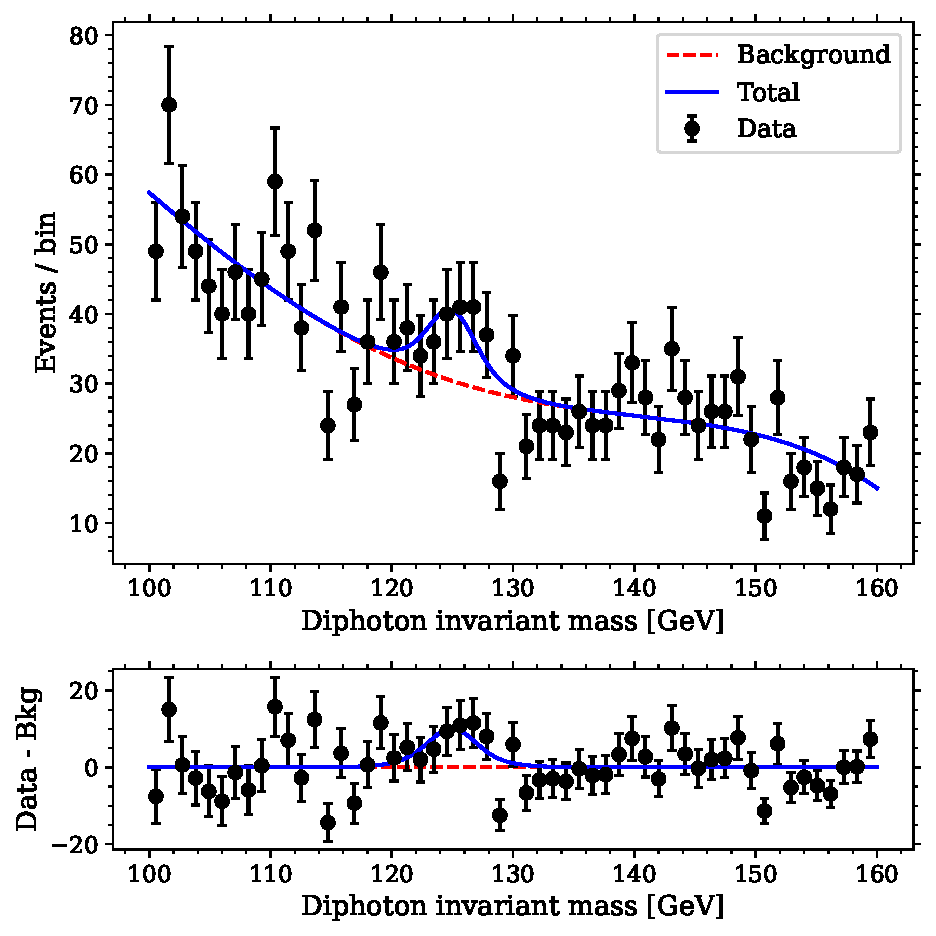
\includegraphics[width=0.6\textwidth]{figures/fit.pdf}
\caption{Fit to the diphoton invariant mass spectrum. \textbf{Top:} The observed data (black points) are shown alongside the fitted background-only model (red) and the full signal+background model (blue). \textbf{Bottom:} Residuals highlighting the excess of events near the Higgs mass.}
\label{fig:fit}
\end{figure}


\begin{figure}[htbp]
\centering
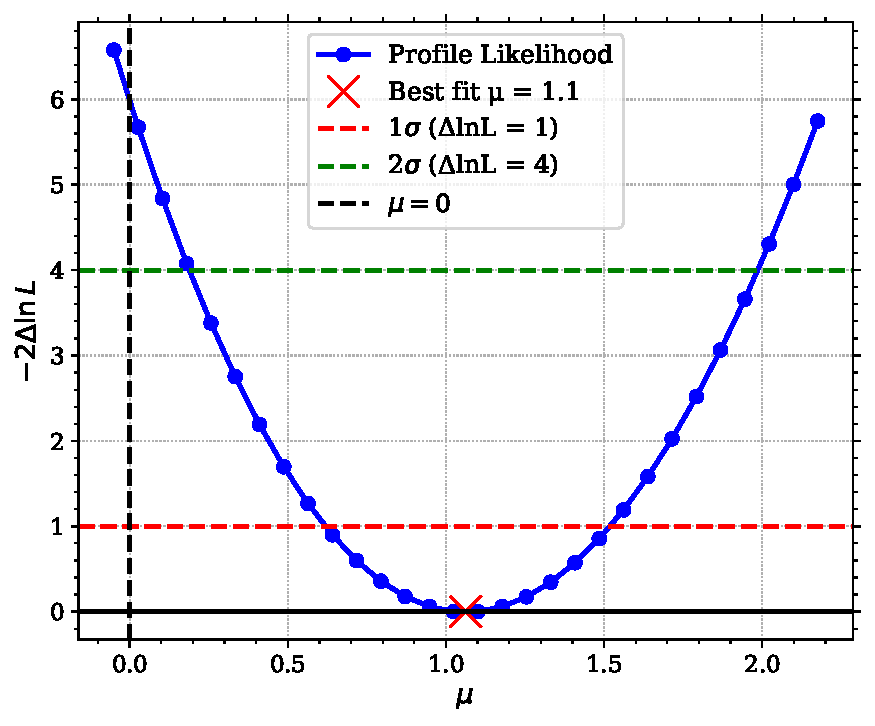
\includegraphics[width=0.5\textwidth]{figures/mu_scan.pdf}
\caption{Profile likelihood scan for the signal strength parameter \( \mu \). The minimum at \( \mu = 1.1 \) (red cross) represents the best-fit value, with uncertainty intervals indicated by the horizontal dashed lines: \( \Delta \ln L = 1 \) (red) and \( \Delta \ln L = 4 \) (green), corresponding approximately to $1\sigma$ and $2\sigma$ confidence levels, respectively. The vertical dashed black line marks the background-only hypothesis (\( \mu = 0 \)).}
\label{fig:mu}
\end{figure}

\subsection*{Results and Significance}

Table~\ref{tab:higgs_results} and Figure~\ref{fig:fit} present the fit results. 

A good fit quality is indicated by a reduced chi-squared value ($\chi^2/\text{ndof}$) of 1.5, which is reasonably close to 1. It might indicate minor imperfections in the model or perhaps slightly underestimated uncertainties in the data bins (which were assumed to be to be $\sqrt{N}$). The residual plot helps confirm this.



The signal strength is extracted via a profile likelihood scan, shown in Figure \ref{fig:mu}, yielding:
\[
\mu = 1.1 \pm 0.4,
\]
within one standard deviation it is consistent with the Standard Model prediction ($\mu=1$), and far from the background-only hypothesis ($\mu=0$).





The test statistic for the likelihood ratio:
\[
\Delta(-2 \ln L) = -2 \ln \left( \frac{L_{bkg}}{L_{s+b}} \right) = (-2 \ln L_{bkg}) - (-2 \ln L_{s+b}).
\]
Based on Wilks' theorem, the significance in terms of standard deviations ($\sigma$) is approximately $\sqrt{\Delta(-2 \ln L)}$. The calculated value is $\Delta(-2 \ln L) = 5.99$, corresponding to a significance of $2.45\sigma$.

A significance of $2.45\sigma$ provides some indication of the presence of the Higgs boson signal in this dataset, but it does not meet the conventional thresholds of $3\sigma$ for an "evidence" claim or $5\sigma$ for a "discovery" claim.



\newpage

\section*{C2\quad Event Classification with Neural Networks}


\section{Event Classification in Particle Physics Detectors}

Event classification involves identifying the underlying physics process responsible for a given event—e.g., distinguishing a Higgs boson decay from background or tagging the flavour of quarks from a hadronic decay. Detectors capture the final-state particles resulting from collisions (such as \( e^-e^+ \rightarrow Z^0 \rightarrow q\bar{q} \)), and the goal is to determine the type of quark produced (e.g., \( b\bar{b}, c\bar{c}, s\bar{s} \), etc.).

Traditionally, classification relied on cut-based selections or shallow multivariate methods. With the advent of machine learning, boosted decision trees (BDTs) became popular. Today, deep learning is shifting the paradigm, with a move towards end-to-end classification. This approach involves feeding \textbf{raw or minimally processed detector data} directly into neural networks, allowing them to learn relevant features automatically. Such methods can capture complex patterns and correlations in the data that may be missed by traditional reconstruction techniques, particularly when working with high-dimensional data and intricate dependencies.


\subsection{Neural Network-Based Classification}

\subsubsection{Theoretical Foundation \cite{rpp2023-machine-learning}}

In classification tasks, the aim is to map detector-derived features \( \mathbf{x} \in \mathcal{X} \) to class labels \( y \in \mathcal{Y} \) (e.g., flavour categories). In the \textbf{binary case}, the Neyman-Pearson lemma gives the optimal discriminator as the likelihood ratio:
\[
    f^*_{\text{N.P.}}(x) = \frac{p(x|y=1)}{p(x|y=0)}.
\]

A neural network trained with mean-squared error (MSE) approximates the \textbf{posterior}:
\[
    f^*_{\text{MSE}}(x) = \mathbb{E}_{p(y|x)}[x] = p(y=1|x) = \frac{p(x|y=1)p(y=1)}{p(x)},
\]
which relates to the likelihood ratio via a \textbf{monotonic} transformation:
\[
    f^*_{\text{N.P.}}(x) = \frac{p(y=0)}{p(y=1)} \cdot \frac{f^*_{\text{MSE}}(x)}{1 - f^*_{\text{MSE}}(x)}.
\]

This transformation \textbf{preserves the receiver operating characteristic (ROC) curve}, making the classification performance invariant to prior probabilities. 

For multi-class problems, neural networks trained with cross-entropy loss approximate the true class posterior \( p(y=c|x) \). However, unlike in binary classification, multi-class outputs depend on the priors \( p(y) \) used during training, and often require \textbf{calibration} if the training data priors (often reflected by class balance) differ from the priors in the application or test scenario.


\subsubsection{Architectures}

Various neural architectures have demonstrated strong performance in event tagging.

One prominent approach is the use of convolutional neural networks (CNNs), which are particularly effective for processing image-like data. Detector data can be represented as images or matrices, allowing CNNs to leverage spatial hierarchies in the input.~\cite{Chekanov_2019, Aurisano_2016}

Graph Neural Networks (GNNs) are another common choice. GNNs are designed to operate on graph-structured data, where nodes represent particles and edges represent interactions or relationships, such as those from the same vertex or jet.~\cite{PhysRevD.110.032008}

Recurrent Neural Networks (RNNs), including variants such as Long Short-Term Memory (LSTM) networks, are tailored for sequential data, making them suitable for time-ordered measurements or ordered particle lists based on criteria such as energy.~\cite{app13053282}

Transformers, which leverage attention mechanisms, are highly effective at capturing long-range dependencies and complex relationships in data.

\textit{ParticleNet} \cite{Qu_2020}, as well as transformer-based architectures such as the \textit{Particle Transformer (ParT)} \cite{qu2024particletransformerjettagging} and the \textit{DeepJetTransformer} \cite{Blekman:2024wyf}, represent state-of-the-art performance in event tagging tasks.

\section{Useful Features for Flavour Tagging}

To distinguish between hadronic decays of the \( Z^0 \) boson into different quark flavours (\( b\bar{b} \), \( c\bar{c} \), and \( s\bar{s} \)), a set of discriminating features can be extracted from the reconstructed event data. The most informative categories in the available data are:

\subsection{Displaced Vertices}

Heavy-flavour quarks, particularly \( b \) and \( c \), form hadrons with relatively long lifetimes. These often result in displaced secondary vertices (SVs) away from the primary vertex (PV). Useful variables include:
\begin{itemize}
  \item \texttt{Vertex\_isPV}: Primary vertex flag (0 or 1).
  \item \texttt{Vertex\_x, y, z} and \texttt{Vertex\_xerr, yerr, zerr}: Spatial coordinates of vertices and their associated uncertainties.
  \item \texttt{Vertex\_ntracks}, \texttt{Vertex\_chi2}, \texttt{Vertex\_m}: Number of tracks, vertex fit quality, and invariant mass of the vertex.
  \item Distance of each particle from the PV (derived from vertex and particle origin data).
\end{itemize}

\subsection{Leptons from Cascade Decays}

Semileptonic decays in the chains \( b \rightarrow c \rightarrow s \) frequently produce muons or electrons. The presence of these leptons is a strong indicator of heavy-flavour content:
\begin{itemize}
  \item \texttt{Particle\_ID}, \texttt{Particle\_q}: Encodes particle species and charge. Also useful in other contexts; for example, the presence of kaons may indicate \( s \)-quark jets.
  \item \texttt{Particle\_pt}, \texttt{Particle\_eta}, \texttt{Particle\_phi}: Kinematic properties of leptons.
\end{itemize}

\subsection{Thrust Axis and Event Geometry}

As the \( Z^0 \) boson is produced at rest, the resulting quarks tend to fly back-to-back. The thrust vector approximates the original quark directions:
\begin{itemize}
  \item \texttt{Thrust\_x, y, z}: Components of the unit thrust vector.
  \item Angle between each particle’s momentum vector and the thrust axis (a derived quantity).
\end{itemize}

\subsection{Global Momentum Characteristics}

Differences in quark mass manifest as variations in the total energy and momentum of the event. Particle and vertex multiplicities also serve as informative indicators. Events containing \( b \)-quarks typically produce more secondary decays, resulting in higher numbers of particles and vertices. Variables such as \texttt{nParticle} and \texttt{nVertex} provide an event-level overview of activity.

In practice, modern neural networks often require only raw or low-level features; even in the absence of hand-crafted, high-level variables, sufficiently powerful architectures can learn the relevant abstractions through optimisation.



\section{Model for Event Classification}


To classify hadronic \( Z^0 \rightarrow q\bar{q} \) decays (\( q \in \{b, c, s\} \)), we design a neural network that integrates event-level global features with variable-length sequences of particles and vertices. The model employs Transformer encoders with \textbf{self-attention} and \textbf{cross-attention} mechanisms, along with attention pooling. These attention mechanisms enable the network to handle \textbf{variable-length} sequences and capture \textbf{contextual relationships}—both among individual objects and between those objects and global event observables.


\subsection{Input Representation}

Each event is represented by three groups of features:

\begin{itemize}
    \item \textbf{Global features:} A fixed-length vector \( \mathbf{g} \in \mathbb{R}^{d_g} \), consisting of:
    \[
    \mathbf{g} = \left[ T_x, T_y, T_z,\ n_{\text{particles}},\ n_{\text{vertices}},\ n_{\text{SV}},\ n_{\text{charged}},\ E_{\text{tot}},\ p_T^{\text{tot}},\ \chi^2_{\text{PV}},\ n_{\text{tracks, PV}} \right]
    \]
    where \( T_{x,y,z} \) are thrust components, and SV denotes secondary vertices.
        
    \item \textbf{Particle features:} A set of vectors \( \mathbf{P} = \{ \mathbf{p}_i \in \mathbb{R}^{d_p} \}_{i=1}^{N_p} \), with \( N_p \leq 25 \), representing individual particles. Each \( \mathbf{p}_i \) includes:
    \[
    \mathbf{p}_i = \left[ p_x, p_y, p_z, E, q, \cos\theta_{\text{thrust}},\ \text{PID encodings},\ \text{charged flag},\ \text{vertex features},\ |\Delta \mathbf{r}_{\text{PV}}| \right]
    \]
    where the PID encodings are one-hot indicators (e.g., kaon, pion, muon, electron, photon), the charged flag indicates whether the particle is charged, vertex features are copied from the associated origin vertex (e.g., position, mass, \(\chi^2\), etc.), and \( |\Delta \mathbf{r}_{\text{PV}}| \) is the displacement from the primary vertex.
    
    \item \textbf{Secondary vertex features:} A sequence \( \mathbf{V} = \{ \mathbf{v}_j \in \mathbb{R}^{d_v} \}_{j=1}^{N_v} \), with \( N_v \leq 4 \). Each vertex vector includes:
    \[
    \mathbf{v}_j = \left[ m,\ \chi^2,\ n_{\text{tracks}},\ x,\ y,\ z \right]
    \]
\end{itemize}



\subsection{Model Structure}

The architecture processes the three input groups via separate branches and then fuses their representations:

\begin{itemize}
    \item \textbf{Global Branch:} The global vector \( \mathbf{g} \) is passed through a \textbf{multi-layer perceptron (MLP)} with dropout:
    \[
    \mathbf{g}' = \mathrm{MLP}_{\text{global}}(\mathbf{g})
    \]

    \item \textbf{Particle Branch:} Each particle \( \mathbf{p}_i \) is linearly projected to an \textbf{embedding space}:
    \[
    \tilde{\mathbf{p}}_i = W_p \mathbf{p}_i + \mathbf{b}_p
    \]
    The embedded sequence \( \tilde{\mathbf{P}} = \{\tilde{\mathbf{p}}_i\} \) is then passed through \( L=3 \) \textbf{Transformer encoder layers} with multi-head self-attention:
    \[
    \mathbf{H}_P = \mathrm{Transformer}_{\text{particles}}^{(L)}(\tilde{\mathbf{P}},\ \mathbf{M}_P)
    \]
    where \( \mathbf{M}_P \) is a binary mask for padding. This allows the model to learn contextualised particle representations, capturing dependencies such as correlations between decay products.
    
    
    Attention pooling is applied:
    \[
    \mathbf{z}_P = \sum_{i} \alpha_i \mathbf{h}_i,\quad \alpha_i = \frac{\exp(\mathbf{w}^\top \mathbf{h}_i)}{\sum_j \exp(\mathbf{w}^\top \mathbf{h}_j)}
    \]

    \item \textbf{SV Branch:} The SV sequence \( \mathbf{V} \) is \textbf{embedded} and passed through \textbf{similar Transformer layers} and attention pooling:
    \[
    \mathbf{H}_V = \mathrm{Transformer}_{\text{SV}}^{(L)}(\tilde{\mathbf{V}},\ \mathbf{M}_V),\quad \mathbf{z}_V = \mathrm{AttnPool}(\mathbf{H}_V)
    \]
\end{itemize}




\subsection{Cross-attention and Fusion}

To allow interaction between global and sequence-derived representations, we introduce a \textbf{cross-attention} mechanism where the global embedding attends over both the particle and SV embeddings. This enables the model to dynamically weigh which particle- or vertex-level features are relevant given the global context.

\[
\mathbf{c}_P = \mathrm{CrossAttn}(\mathbf{g}',\ \tilde{\mathbf{P}},\ \mathbf{M}_P), \quad
\mathbf{c}_V = \mathrm{CrossAttn}(\mathbf{g}',\ \tilde{\mathbf{V}},\ \mathbf{M}_V)
\]

The final event representation is a \textbf{concatenation} of all processed vectors:
\[
\mathbf{z} = \left[ \mathbf{g}',\ \mathbf{z}_P,\ \mathbf{z}_V,\ \mathbf{c}_P,\ \mathbf{c}_V \right]
\]
This vector is passed through additional \textbf{dense layers} to produce the final output:
\[
\hat{\mathbf{y}} = \mathrm{softmax} \left( \mathrm{MLP}_{\text{final}}(\mathbf{z}) \right),\quad \hat{\mathbf{y}} \in \mathbb{R}^3
\]
representing the probabilities of \( Z \rightarrow b\bar{b} \), \( c\bar{c} \), and \( s\bar{s} \) decays.

\begin{table}[htbp]
\centering
\begin{tabular}{lcccc}
\hline
\textbf{Class} & \textbf{Precision} & \textbf{Recall} & \textbf{F1-Score} & \textbf{Support} \\
\hline
b-event & 0.962 & 0.961 & 0.962 & 29,710 \\
c-event & 0.934 & 0.934 & 0.934 & 29,968 \\
s-event & 0.969 & 0.970 & 0.969 & 31,854 \\
\hline
Accuracy & & & 0.955 & 91,532 \\
Macro avg & 0.955 & 0.955 & 0.955 & 91,532 \\
Weighted avg & 0.955 & 0.955 & 0.955 & 91,532 \\
\hline
\end{tabular}
\caption{Classification performance metrics on test data.}
\label{tab:classification_results}
\end{table}

\begin{figure}[!h]
    \centering
    
\includegraphics[width=0.75\linewidth]{report/figures/training_curves.pdf}
    \caption{Training and validation performance over 50 epochs. Left: Accuracy curves, showing steady and converging improvement for both training and validation sets. Right: Loss curves, indicating a consistent decrease in training and validation loss. The drop around epoch 40 reflects a learning rate reduction (from 0.001 to 0.0005). No signs of overfitting are evident, and continued training could yield additional gains.}
    \label{fig:training_validation_metrics}
\end{figure}



\subsection{Results}


The model is trained for \inlinecode{epochs=50}, with a \inlinecode{batch\_size=256} and \inlinecode{lr\_patience=10}. Dropout layers are incorporated throughout the network to mitigate overfitting. The training curves are presented in Figure~\ref{fig:training_validation_metrics}. Accuracy on both the training and validation sets exceeds 95\%, although the learning trajectory suggests that the model has not yet fully converged. Further improvements may be achievable through extended training or fine-tuning.

The model is subsequently evaluated on the held-out test set. Test accuracy surpasses 95\% as well, indicating strong generalisation performance. Detailed classification metrics are summarised in Table~\ref{tab:classification_results}.

\begin{figure}[htbp]
    \centering
    
\includegraphics[width=0.95\linewidth]{report/figures/prob_histograms.pdf}
    \caption{Histograms of predicted class probabilities for events with true labels of b, c, and s. Each subplot shows the distribution of predicted probabilities across all classes. Solid bars represent training data, and dashed lines denote test data. Clear separation of the correct class from the others indicates strong class discrimination, while close overlap between training and test curves suggests robust generalisation.}
    \label{fig:prob_hists}
\end{figure}


\begin{figure}[!h]
    \centering
    
\includegraphics[width=0.75\linewidth]{report/figures/roc_pr_curves.pdf}
    \caption{Performance evaluation on the test set using ROC (left) and Precision-Recall (right) curves for each class (b, c, s). The high AUC scores in the ROC plots demonstrate excellent classification performance. The PR curves further confirm strong precision and recall across classes, particularly important for handling class imbalance.}
    \label{fig:roc_pr_curves}
\end{figure}


Figure~\ref{fig:prob_hists} shows the predicted class probability distributions for each true class. The near-identical shapes of the distributions for training and test sets indicate minimal overfitting and suggest that the training and test datasets have similar underlying distributions. Furthermore, the sharp separation between the predicted probability for the true class (peaked near 1) and the other classes (clustered near 0) demonstrates the model’s strong discriminative capability.



To further quantify classification performance, Receiver Operating Characteristic (ROC) and Precision-Recall (PR) curves are shown in Figure~\ref{fig:roc_pr_curves}. All classes exhibit AUC scores 0.99, confirming excellent sensitivity and precision, even in the presence of class imbalance.


\section{Conclusion}

In this study, we have demonstrated the effectiveness of a transformer-based neural network architecture for classifying hadronic \( Z^0 \rightarrow q\bar{q} \) events by quark flavour. The model integrates global event observables with structured particle- and vertex-level data, employing attention mechanisms—both self-attention and cross-attention—to capture intricate dependencies and contextual relationships within and across data modalities.

Our results indicate a high level of performance, with classification accuracies exceeding 95\% and AUC scores above 0.99 for all classes. The consistency between training and test distributions, as observed from the probability histograms, highlights the strong generalisation capacity of the model and minimal signs of overfitting. This robustness is further supported by the training dynamics and performance curves over multiple epochs.

Perhaps most importantly, the model’s ability to learn directly from low-level, minimally processed features underscores the strength of deep learning in handling the complexities of particle physics data. Owing to these advantages, neural networks present a powerful, flexible, and scalable solution for event classification tasks—paving the way for their broader adoption in experimental analyses across high-energy physics.



\clearpage
\newpage
\appendix
\section{Use of AI Tools}
In this report, AI tools were utilised to enhance the quality and presentation of the content. Their contributions include:

\begin{itemize}
    \item \textbf{Literature Review} - Utilised “Deep research” (OpenAI) and “DeepSearch” (xAI) for high-level overviews and literature searches.
    
    \item \textbf{Drafting} – Assisted in writing various sections of the report, particularly mathematical derivations and expressions, as well as the Conclusion section of C2, and Appendix. AI tools were also used to generate captions for figures and tables.
    
    \item \textbf{Proofreading} – Reviewed grammar, improved sentence structure, and suggested alternative wordings to enhance clarity and coherence throughout the report.
    
    \item \textbf{LaTeX Assistance} – Helped resolve issues encountered during the LaTeX formatting process, including debugging compilation errors and formatting well-structured tables based on the provided data.
\end{itemize}



\section{Template Information}
This report was formatted using the LaTeX template provided in the Example Coursework by Michal Dorko, with some modifications applied.


\newpage
\printbibliography
\end{document}